% CMPE 258 talk (10 min, Thu Dec 3). Beamer, compiled with tectonic (conda env `paper`).
% Every number comes from reports/final_eval/ (test) or an earlier logged run (labelled "development").
\documentclass[aspectratio=169,11pt]{beamer}
\usetheme{default}
\usecolortheme{dove}
\setbeamertemplate{navigation symbols}{}
\setbeamertemplate{footline}[frame number]
\usepackage{tikz}
\usetikzlibrary{arrows.meta,positioning,shapes.geometric}
\usepackage{booktabs}
\definecolor{acc}{HTML}{C44E52}
\definecolor{blu}{HTML}{4C72B0}
\definecolor{gr}{HTML}{7F7F7F}
\setbeamercolor{frametitle}{fg=blu}
\newcommand{\src}[1]{\vfill{\tiny\color{gr}#1}}

\title{Which part should the planner try next?}
\subtitle{Cost-aware query ordering for assembly-by-disassembly\\with a tight-clearance SE(3) planner}
\author{Aaron Chandler}
\institute{CMPE 258 Deep Learning, San Jos\'e State University}
\date{December 3, 2026}

\begin{document}

\begin{frame}
\titlepage
\end{frame}

% 1 ------------------------------------------------------------------ application
\begin{frame}{Automated disassembly asks the same question again and again}
\begin{columns}
\column{0.55\textwidth}
\begin{itemize}
\item Recycling and teardown (e.g.\ battery modules) need a \textbf{removal sequence} for real CAD products.
\item Assembly-by-disassembly: at each step, ask a motion planner \emph{``can part $i$ come out?''}
\item Each question is a \textbf{CMG-RRT query} in SE(3): \textcolor{blu}{0.04\,s} if a straight pull works,
\textcolor{acc}{30\,s} if it times out.
\item A timeout is \emph{not} a proof that the part is stuck: it is a \textbf{censored} observation.
\end{itemize}
\column{0.45\textwidth}
\centering
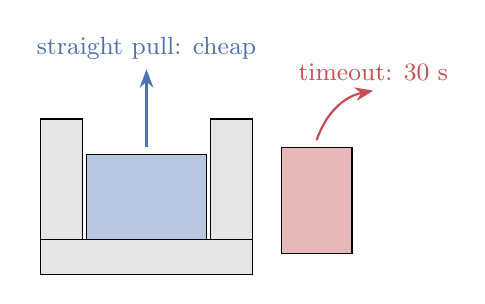
\begin{tikzpicture}[scale=0.9]
\draw[fill=gr!20] (0,0) rectangle (3,0.5);
\draw[fill=gr!20] (0,0.5) rectangle (0.6,2.2);
\draw[fill=gr!20] (2.4,0.5) rectangle (3,2.2);
\draw[fill=blu!40] (0.65,0.5) rectangle (2.35,1.7);
\draw[-{Stealth},thick,blu] (1.5,1.8) -- (1.5,2.9) node[above]{\small straight pull: cheap};
\draw[fill=acc!40] (3.4,0.3) rectangle (4.4,1.8);
\draw[-{Stealth},thick,acc] (3.9,1.9) to[bend left] (4.7,2.6) node[above]{\small timeout: 30 s};
\end{tikzpicture}
\end{columns}
\src{Oracle v2 query costs: run 04 T4 (\texttt{reports/run04/oracle\_v2.md}); median 0.037\,s on the validation set.}
\end{frame}

% 2 ------------------------------------------------------------------ problem
\begin{frame}{The exact problem: order the queries to reach the first success cheaply}
\[
C(\pi;S)=\sum_{k} t_{\pi_k}\prod_{j<k}(1-y_{\pi_j})
\qquad\text{(planner time until the first removable part)}
\]
\begin{itemize}
\item Optimal for independent tests: query in descending $p_i/c_i$ (Simon \& Kadane, 1975).
\item $p_i$ = P(success within $T$), $c_i$ = expected (censored) query cost $\mathbb{E}[\min(t_i,T)]$.
\item Constraints: the ranker runs once per state on a CPU and must cost far less than one query.
\end{itemize}
\end{frame}

% 3 ------------------------------------------------------------------ landscape
\begin{frame}{Existing approaches learn \emph{whether} a part comes out, not \emph{what it costs}}
\begin{center}\footnotesize
\begin{tabular}{lll}
\toprule
& predicts & tester \\
\midrule
Cebulla et al.\ (ICRA 2023) & removability & discrete / simulated \\
ASAP (ICRA 2024), open source & next removable part (GNN) & physics simulator \\
CMG-RRT (WAFR 2026), open source & --- (planner) & SE(3), tight clearance \\
\textbf{This project} & \textbf{P(success) and censored cost} & \textbf{CMG-RRT} \\
\bottomrule
\end{tabular}
\end{center}
\begin{itemize}
\item Gap: no model of query \textbf{cost}, or of \textbf{timeouts as censored data}, for a rotational planner.
\end{itemize}
\end{frame}

% 4 ------------------------------------------------------------------ pipeline
\begin{frame}{What we built}
\centering
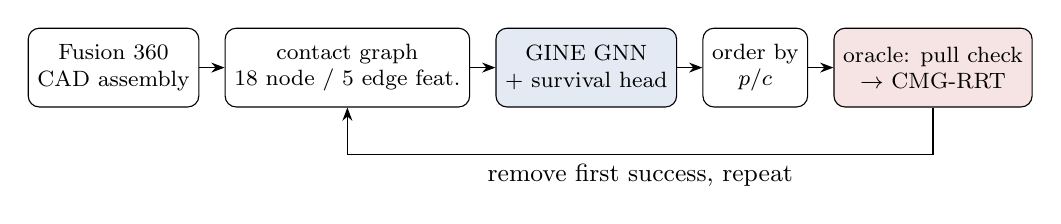
\begin{tikzpicture}[node distance=0.55cm and 0.32cm, box/.style={draw,rounded corners,align=center,font=\footnotesize,minimum height=1.0cm,fill=white}]
\node[box] (cad) {Fusion 360\\CAD assembly};
\node[box,right=of cad] (g) {contact graph\\18 node / 5 edge feat.};
\node[box,right=of g,fill=blu!15] (gnn) {GINE GNN\\+ survival head};
\node[box,right=of gnn] (rank) {order by\\$p/c$};
\node[box,right=of rank,fill=acc!15] (orc) {oracle: pull check\\$\rightarrow$ CMG-RRT};
\draw[-{Stealth}] (cad) -- (g); \draw[-{Stealth}] (g) -- (gnn); \draw[-{Stealth}] (gnn) -- (rank); \draw[-{Stealth}] (rank) -- (orc);
\draw[-{Stealth}] (orc.south) -- ++(0,-0.6) -| node[pos=0.25,below,font=\small]{remove first success, repeat} (g.south);
\end{tikzpicture}
\vspace{0.4cm}
\begin{itemize}\small
\item Survival head: hazard in 8 log-spaced bins up to $T=30$\,s, censoring-aware likelihood $\Rightarrow$ both $p$ and $c$.
\item Ablations: MLP (no message passing), BCE head ($p$ only), PointNet features, tail-aware loss.
\item Baselines: random, outside-in, fewest contacts, ASAP zero-shot, ASAP retrained.
\end{itemize}
\end{frame}

% 5 ------------------------------------------------------------------ data
\begin{frame}{Data: valid states from known feasible disassemblies (course feedback)}
\begin{itemize}
\item Start from the real assembled product; query \textbf{every} part; remove a verified success; repeat.
\item 2,022 assemblies, 3--12 parts, \textbf{41,913 labelled queries}, 12.6\,h on 10 cores, idle-guarded timing.
\item Oracle fixed first: the original adapter never tried the straight pull from the start pose (123/124 misses),
and 18.5\% of its successes went through parts at fine resolution.
\item Pre-registered protocol; \textbf{fresh test set} of 347 assemblies (51\% with 9--12 parts), evaluated once.
\end{itemize}
\src{\texttt{reports/run04/REPORT.md}, \texttt{docs/PREREG\_run05.md}, \texttt{data/splits/v2\_split.json}.}
\end{frame}

% 6 ------------------------------------------------------------------ main result
\begin{frame}{Test result: cheaper than ASAP and random, ties the contact heuristic}
\centering
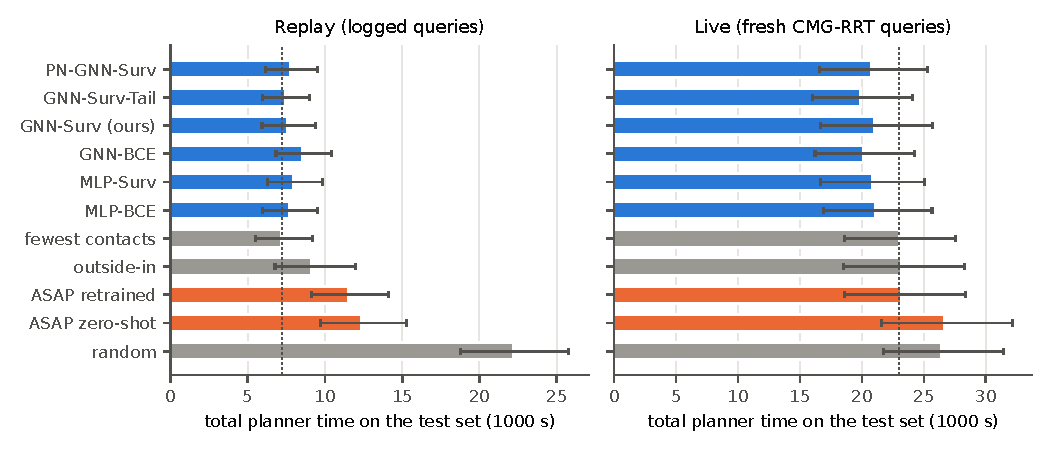
\includegraphics[width=0.94\linewidth]{figures/totals_replay_live.pdf}\\[-1pt]
{\scriptsize\color{gr} blue: ours \quad orange: ASAP \quad gray: untrained; dashed: fewest contacts}\\[3pt]
\small GNN-Surv / fewest contacts: replay $1.055$ [0.887, 1.257], live $0.915$ [0.819, 1.015] $\Rightarrow$
\textcolor{acc}{\textbf{does not beat}} (pre-registered rule, both).
\src{\texttt{reports/final\_eval/replay.md}, \texttt{live.md}; bootstrap over 341/347 assemblies; 5 seeds per model.}
\end{frame}

% 7 ------------------------------------------------------------------ ablations
\begin{frame}{Ablations on test: the cost-aware head helps --- but not robustly}
\begin{center}\footnotesize
\begin{tabular}{lcc}
\toprule
contrast (ratio of total time, A/B) & ratio [95\% CI] & Holm $p$\\
\midrule
\textbf{survival $p/c$ vs BCE $p$} (GNN) & \textbf{0.887} [0.785, 0.999] & $6\times10^{-7}$\\
GNN-Surv vs ASAP retrained & 0.660 [0.543, 0.793] & $5\times10^{-7}$\\
GNN vs MLP (survival) & 0.951 [0.831, 1.084] & 0.55\\
hand-made features vs + PointNet (GNN-Surv vs PN-GNN-Surv) & 0.977 [0.871, 1.091] & 1\\
plain vs tail-aware loss (GNN-Surv vs GNN-Surv-Tail) & 1.024 [0.934, 1.112] & 1\\
\bottomrule
\end{tabular}
\end{center}
\begin{itemize}\small
\item Survival vs BCE holds in replay; on the clean subset the CI reaches 1.001, live it is cheaper only per assembly, and the MLP pair goes the other way.
\item Validation favoured the most-tuned variants; cross-validation and test did not confirm them.
\end{itemize}
\src{\texttt{reports/final\_eval/REPORT.md} \S2; \texttt{reports/explore/cv.md}.}
\end{frame}

% 8 ------------------------------------------------------------------ live (placeholder)
\begin{frame}{Live: fresh CMG-RRT queries, 347 full disassemblies per method}
\begin{itemize}
\item 17,697 disassembly runs, idle-guarded; every confounded run re-run, none left confounded.
\item GNN-Surv / fewest contacts $=\mathbf{0.915}$ [0.819, 1.015], Holm $p=0.13$: \textcolor{acc}{\textbf{does not beat}} (same verdict as replay).
\item Cheaper than ASAP zero-shot (0.789) and ASAP retrained (0.906 [0.827, 0.994]) live, too.
\item Exploratory: GNN-Surv + ListNet loss 0.797 vs fewest contacts live --- but not in replay, so: a lead, not a result.
\end{itemize}
\src{\texttt{reports/final\_eval/live.md}; seed-mean of 5 seeds per trained model (pre-registered).}
\end{frame}

% 9 ------------------------------------------------------------------ budget policy
\begin{frame}{The biggest win was not learned: try 3 s first}
\begin{itemize}
\item Two-pass policy: every part gets 3\,s; only if none comes out, retry at 30\,s.
\item Fewest contacts: 7,202\,s $\rightarrow$ \textbf{2,008\,s} ($-72\%$) on test; GNN-Surv 7,595\,s $\rightarrow$ 1,904\,s.
\item Under the same policy, learned vs heuristic: 0.948 [0.820, 1.095] --- no detectable difference.
\item Live: about $-50\%$ (stuck runs pay the retry; the planner overruns short budgets).
\end{itemize}
\centering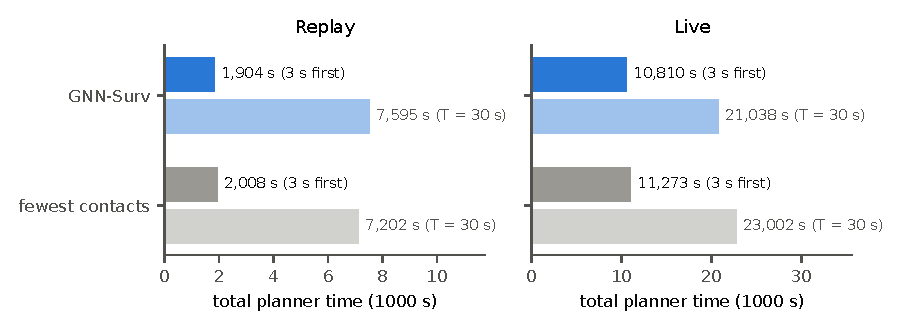
\includegraphics[width=0.78\linewidth]{figures/budget_policy.pdf}
\src{Exploratory (post-registration, chosen on validation): \texttt{reports/final\_eval/replay.md}.}
\end{frame}

% 10 ----------------------------------------------------------------- latency
\begin{frame}{Cost of the ranker vs the planner time at stake}
\begin{itemize}
\item GNN-Surv: 32k parameters, 0.12\,ms per state (1 CPU thread) + 2.4\,ms features.
\item ASAP's model: 1.7M parameters, 7.0\,ms per state.
\item One avoided timeout = 30\,s = $\sim$12,000 ranker calls.
\end{itemize}
\src{\texttt{reports/run05/profile.md} (timing flagged confounded by the idle-guard rule; outside load $\le$0.36 cores).}
\end{frame}

% 11 ----------------------------------------------------------------- failure analysis
\begin{frame}{Why it fails on test: confident timeouts on big assemblies}
\begin{columns}
\column{0.58\textwidth}
\begin{itemize}\small
\item 89\% of fewest contacts' total is in its costliest 5\% of states (77\% for GNN-Surv).
\item GNN-Surv's loss vs fewest contacts: \textbf{85 states where it queried a timeout first} (+3,153\,s).
\item In its costliest states it predicted $p\approx0.9$--$1.0$, $c\le3.7$\,s for parts that then ran 30\,s.
\item Shift: training is 79\% 3--8-part assemblies; test is 51\% 9--12-part and 63\% interpenetrating CAD.
\end{itemize}
\column{0.42\textwidth}
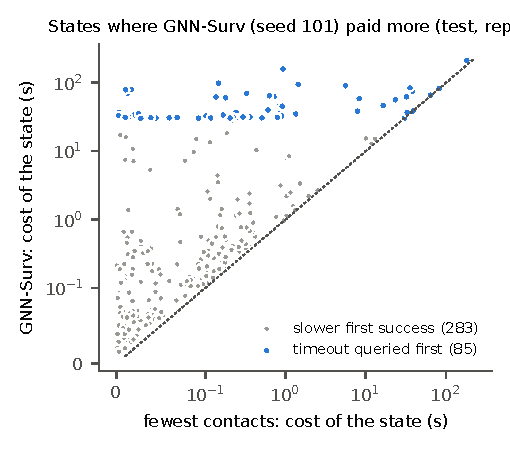
\includegraphics[width=\linewidth]{figures/failure_scatter.pdf}
\end{columns}
\src{\texttt{reports/final\_eval/failure\_analysis.md}.}
\end{frame}

% 12 ----------------------------------------------------------------- negative results / insights
\begin{frame}{Negative results and what we learned}
\begin{itemize}
\item The planner adapter was the first bug: start pose never tested, coarse goal check (18.5\% invalid paths).
\item A learned SDF ``solved'' a tight puzzle 3/3 --- every path went through the part (exact check: 0/3).
\item 95--98\% of successes are straight pulls; CMG-RRT decides the rest, and the timeouts dominate cost.
\item Validation optimism is real: pick on val, confirm out of sample, pre-register the test.
\end{itemize}
\src{\texttt{reports/run04/oracle\_v2.md}, \texttt{sdf\_puzzles.md}, \texttt{labels\_v2.md}; \texttt{reports/run05/REPORT.md}.}
\end{frame}

\begin{frame}{Summary}
\begin{itemize}
\item Cost-aware ordering is cheaper than both ASAP baselines on a fresh test set; its edge over removability-only ordering holds in replay but not robustly.
\item It does not beat a simple contact heuristic on larger, unseen assemblies --- confident timeouts are the reason.
\item A 3\,s first-pass budget cuts planner time by 72\% for every ordering.
\item Next: calibrate for shift (train on 9--12-part assemblies), learn per-part budgets from the survival curve.
\end{itemize}
\vfill
{\small Code: \texttt{github.com/AaronChandler976/curved-path-puzzle-solver}}
\end{frame}

\appendix
\begin{frame}{Backup: a real disassembly with the learned order}
\centering
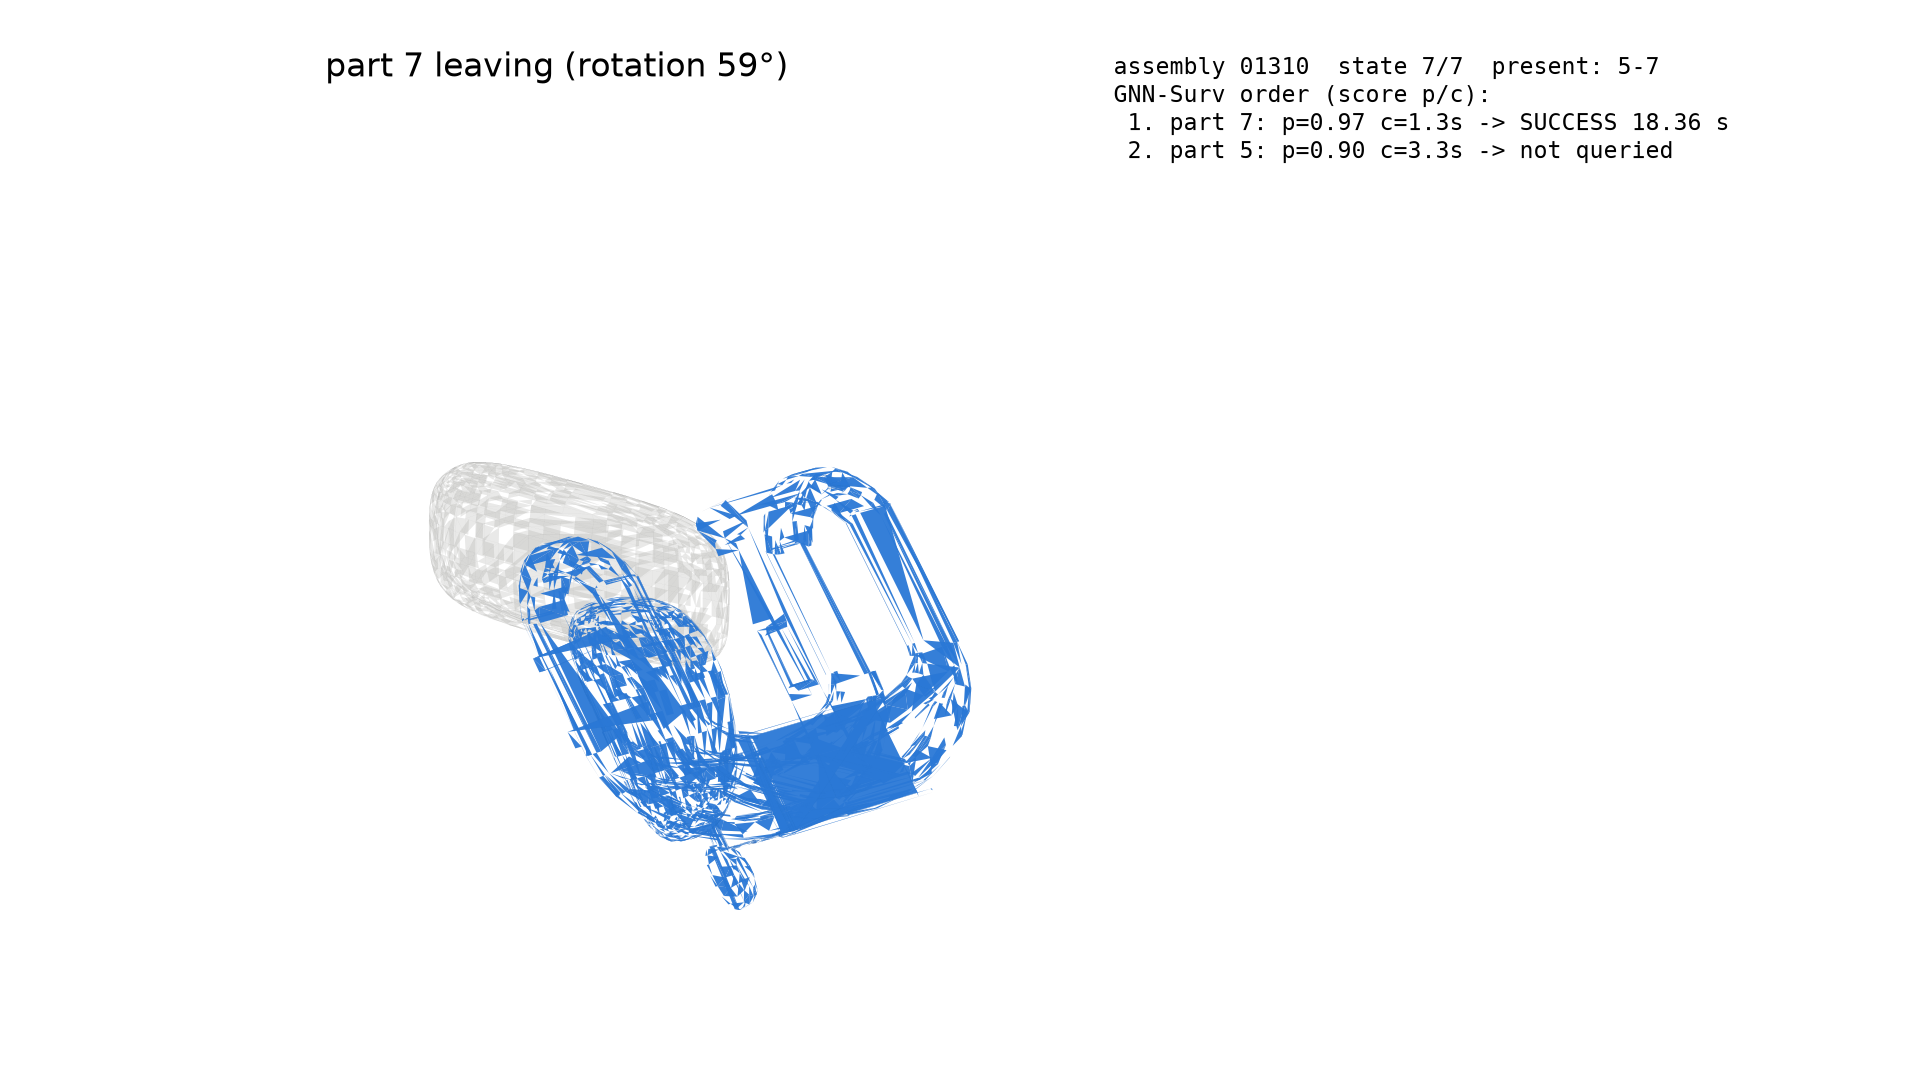
\includegraphics[width=0.72\linewidth]{figures/demo_frame.png}\\
{\small Test assembly 01310, GNN-Surv order; part 7 leaves with a 102° CMG-RRT rotation. Animation: \texttt{talk/demo.mp4}.}
\end{frame}
\end{document}
